% Author: Izaak Neutelings (Februari 2024)
% Description: Event topology of two taus.
\documentclass[border=3pt,tikz]{standalone}
\usepackage{amsmath}
%\usetikzlibrary{calc}
%\usetikzlibrary{decorations.pathmorphing} % for snakes
\usetikzlibrary {shapes.geometric} % for star
\usetikzlibrary{bending} % for arrow head angle
\usetikzlibrary{angles,quotes} % for pic (angle labels)
\usetikzlibrary{arrows.meta} % for arrow size

% COLORS
\colorlet{myred}{red!75!black}
\colorlet{myblue}{blue!70!black}
%\colorlet{mydarkblue}{blue!50!black}
%\colorlet{mygreen}{green!60!black}
\colorlet{myorange}{orange!70!yellow!90!black}

% STYLES
\tikzset{
  >=latex, % for LaTeX arrow head
  pv/.style={myorange!70!red,fill=myorange!60!yellow,line width=0.3,star,star points=7,
             star point height=8pt,minimum size=2pt,draw,scale=0.3*#1},
  pv/.default=1,
  track/.style={-{Latex[scale=0.7]},line width=0.6,myorange!40,line cap=round},
  lepton/.style={track,->,line width=0.9,myred},
  %dashed track/.style={->,mygreen,line width=0.6,line cap=round,
  %                     dash pattern=on 2.3 off 2.0},
  %part/.style={circle,ball color=#1,text=#1!30!black,
  %             postaction={fill=#1!77,fill opacity=0.8,
  %             draw=#1!60!black!90,thin}]},
  %mysmallarrow/.style={-{Latex[length=4.2,width=3.5]},mygreen,thick},
  angarr/.style={{Latex[flex'=1,length=3.2,width=2.8]}-{Latex[flex'=1,length=3.2,width=2.8]}},
}


\begin{document}


% DITAU (exclusive signal for g-2)
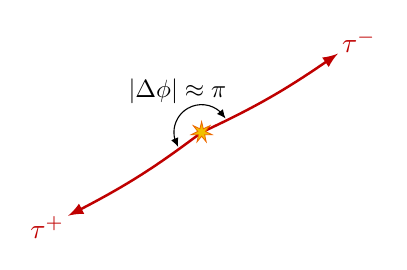
\begin{tikzpicture}
  \def\ang{30} % offset angle of dilepton
  \def\L{2.0} % length tracks
  \coordinate (PV) at (0,0);
  \coordinate (T1) at (\ang:\L);
  \coordinate (T2) at (\ang+182:\L);
  
  % LEPTONS
  \draw[lepton] (PV) to[bend right=5] (T1)
    node[anchor=\ang-180,inner sep=1pt] {$\tau^-$};
  \draw[lepton] (PV) to[bend left=5] (T2)
    node[anchor=\ang,inner sep=1pt] {$\tau^+$};
  
  % ANGLE
  \draw pic[angarr,"$|\Delta\phi|\approx\pi$",draw,angle eccentricity=1,
            angle radius=10pt,pic text options={scale=0.9,shift={(\ang+90:8pt)}}]
    {angle = T1--PV--T2};
  
  % PV
  \node[pv] at (PV) { };
  
\end{tikzpicture}


% DITAU (background for g-2)
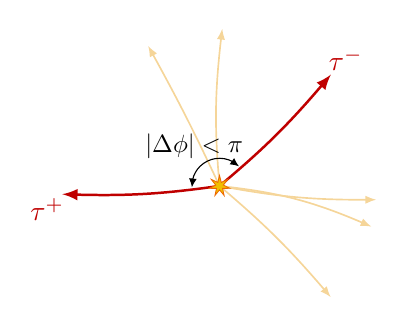
\begin{tikzpicture}
  \def\ang{45} % offset angle of dilepton
  \def\L{2.0} % length tracks
  \coordinate (PV) at (0,0);
  \coordinate (T1) at (\ang:\L);
  \coordinate (T2) at (\ang+138:\L);
  
  % TRACKS
  \foreach \tang [evaluate={\b=10*rand;}] in {44,72,-50,-60,-90}{
    \draw[track] (PV) to[bend right=\b] (\ang+\tang:\L);
  }
  
  % LEPTONS
  \draw[lepton] (PV) to[bend right=5] (T1)
    node[anchor=\ang-180,inner sep=1pt] {$\tau^-$};
  \draw[lepton] (PV) to[bend left=5] (T2)
    node[anchor=\ang,inner sep=1pt] {$\tau^+$};
  
  % ANGLE
  \draw pic[angarr,"$|\Delta\phi|<\pi$",draw,angle eccentricity=1,
            angle radius=10pt,pic text options={scale=0.9,shift={(\ang+90:8pt)}}]
    {angle = T1--PV--T2};
  
  % PV
  \node[pv] at (PV) { };
  
\end{tikzpicture}


% DIMUON N_tracks
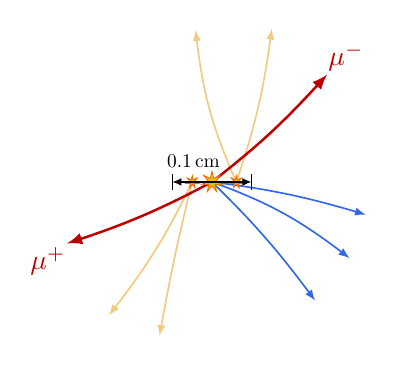
\begin{tikzpicture}
  \def\ang{43} % offset angle of dilepton
  \def\L{2.0} % length tracks
  \def\w{1.0} % width window
  \def\h{0.1} % height measure ticks
  \coordinate (PV) at (0,0);
  \coordinate (V1) at (-0.25*\w,0);
  \coordinate (V2) at ( 0.31*\w,0);
  \coordinate (T1) at (\ang:\L);
  \coordinate (T2) at (\ang+160:\L);
  
  % PU TRACKS
  \foreach \v/\tang [evaluate={\b=10*rand;}] in {1/-165,1/-145,2/34,2/62}{
    \draw[track,myorange!50] (V\v) to[bend right=\b]++ (\ang+\tang:\L);
  }
  
  % HS TRACKS
  \foreach \tang [evaluate={\b=10*rand;}] in {-55,-72,-92}{
    \draw[track,blue!70!cyan!88!black!80] (PV) to[bend right=\b] (\ang+\tang:\L);
  }
  
  % LEPTONS
  \draw[lepton] (PV) to[bend right=5] (T1)
    node[anchor=\ang-180,inner sep=1pt] {$\mu^-$};
  \draw[lepton] (PV) to[bend left=5] (T2)
    node[anchor=\ang,inner sep=1pt] {$\mu^+$};
  
  % VERTICES
  \node[pv] at (PV) { };
  \node[pv=0.6] at (V1) { };
  \node[pv=0.6] at (V2) { };
  
  % measure
  \draw[angarr,thin] (-\w/2,0) coordinate(W1) -- (\w/2,0) coordinate(W2);
  \draw[thin]
    (W1)++(0,-\h) --++ (0,2*\h) node[anchor=-148,scale=0.7] {0.1\,cm} %{1\,cm}
    (W2)++(0,-\h) --++ (0,2*\h);
  
\end{tikzpicture}


\end{document}